\section{Localization of surrounding polygons}\label{c01-c1-localization-of-surrounding-polygons}

We pass from the cylinder observable to polygons surrounding one face in the
plane. Write \(Z(R)\) for the planar gas at fugacity 2 of mutually disjoint
honeycomb polygons enclosing the face center 0 and contained within distance
\(R\) of it. Changing the disk cutoff by a fixed factor will not affect the
exponent.

\begin{proposition}\label{prop:pv:planar-localization}
The disk partition function satisfies
\[
 Z(R)=R^{1/12+o(1)}.
\]
\end{proposition}

There are two comparisons with the balanced cylinder of circumference
\(p=2n\). Two small disk systems, one near each marked face, give the upper
bound directly from \(F_n(2)=n^{1/6+o(1)}\). For the lower bound we must remove
the cylinder polygons that cannot be put into two disk systems of radius
\(p^{1+\delta}\), for fixed \(\delta>0\). These are the essential polygons
and the contractible polygons with oversized planar lifts. We will show that
their total single-polygon weight is bounded, so removing them costs only a
bounded multiplicative factor. The difficulty is the second family: a
contractible polygon may travel far before meeting a horizontal translate.

\subsection{Weighted incompatibility from the zero-free disk}

Let \(r_0>0\) be a common radius of a zero-free disk for \(F_n(\eta)\) about
\(\eta=0\). Available polygons on a fixed balanced cylinder have weights
\(w(P)=x_*^{|P|}\). Write \(I(P,Q)\) for incompatibility, including
\(I(P,P)=1\).

\begin{lemma}\label{lem:pv:weighted-degree}
For every nonempty finite family \(\mathcal H\) of available polygons,
\[
 M_{\mathcal H}=\sum_{P\in\mathcal H}w(P),\qquad
 d_{\mathcal H}
 =\frac{\sum_{P,Q\in\mathcal H}w(P)I(P,Q)w(Q)}{M_{\mathcal H}}
 \le r_0^{-1}.
\]
In particular, the bound does not depend on the circumference or the family.
\end{lemma}

\begin{proof}
The formal logarithm of a hard-core gas is the connected-graph expansion;
see Fern\'andez and Procacci~\cite[Eqs.~(2.2)--(2.4)]{FernandezProcacci2007}.
For a tuple \((P_1,\ldots,P_k)\), its incompatibility graph has the distinct
tuple positions as vertices, even when polygons repeat. Its contribution to
the coefficient of \(\eta^k\) in \(\log F_n(\eta)\) is
\(\prod_iw(P_i)/k!\) times the alternating sum over its connected spanning
edge sets. This follows by expanding the products of \(1-I\) and grouping
components. Finite total polygon weight makes the sums absolutely finite
coefficientwise.

The alternating sum, multiplied by \((-1)^{k-1}\), counts acyclic
orientations with unique source at vertex 1, by the fixed-root
chromatic-polynomial identity of Greene and
Zaslavsky~\cite[Theorem~7.3]{GreeneZaslavsky1983}. In particular, all tuples
contribute with the same sign. One can check the identity by
deletion--contraction at edges incident to the root: the alternating sum is
the linear chromatic coefficient, and the orientation count has the same
addition rule. Delete a root edge when its other endpoint has another
incoming edge; contract it otherwise. These give the corresponding rooted
orientations, with parallel edges simplified, and the recursion ends at the
isolated-root base cases.

Every Hamilton path starting at vertex 1 supplies one such orientation, by
orienting all edges in its path order. Different paths give different
orientations, since the directed Hamilton path forces the total order.
Summing the \((k-1)!\) orders of the remaining tuple positions therefore gives
\begin{equation}\label{eq:pv:degree-coefficient}
 \bigl|[\eta^k]\log F_n(\eta)\bigr|
 \ge \frac1k
 \sum_{P_1,\ldots,P_k\in\mathcal H}
 \prod_{i=1}^k w(P_i)
 \prod_{i=1}^{k-1}I(P_i,P_{i+1}).
\end{equation}
Thus a log coefficient bounds a weighted walk count in the incompatibility
graph, not merely the mass of individual incompatible pairs.

For completeness, use the weighted inner product
\(\langle f,g\rangle_w=\sum_{P\in\mathcal H}w(P)f(P)g(P)\) and the symmetric
operator
\[
 (Af)(P)=\sum_{Q\in\mathcal H}I(P,Q)w(Q)f(Q).
\]
The sum in \eqref{eq:pv:degree-coefficient} is
\(\langle\mathbf1,A^{k-1}\mathbf1\rangle_w\). For odd \(k\), the spectral
moment inequality for the even power \(k-1\) gives
\[
 \langle\mathbf1,A^{k-1}\mathbf1\rangle_w
 \ge M_{\mathcal H}d_{\mathcal H}^{\,k-1}.
\]
Now freeze both \(\mathcal H\) and its containing cylinder, and let odd
\(k\) tend to infinity. Since \(\log F_n\) is analytic in \(|\eta|<r_0\),
its coefficient root growth is at most \(r_0^{-1}\), proving the lemma.
Only the radius is uniform here; no uniformity in \(k\) is required of the
fixed-order \(O_k(1+\log n)\) coefficient bounds.
\end{proof}

To use this lemma for oversized polygons, we will force incompatibilities
between two such polygons after rotating one of them. If all six rotations
of the smaller polygon were compatible with the larger one, their interiors
would all lie inside its period-free interior. The next geometric lemma
rules this out at radius greater than \(p^{1+\delta}\).

\subsection{The six-rotation radius bound}

Write \(\omega=e^{i\pi/3}\) and \(\Lambda=\mathbb Z[\omega]\) for the
triangular face-center lattice.

\begin{lemma}\label{lem:pv:six-rotations}
Let \(V\) be the open Jordan interior of a honeycomb polygon \(Q\) enclosing
0. Suppose that an open set \(U\) contains \(\omega^rV\) for
\(0\le r\le5\), and that
\[
 U\cap(U+kp)=\varnothing\qquad(k\in\mathbb Z\setminus\{0\})
\]
for \(p\ge1\). If \(D=\max_{z\in Q}|z|\), then
\[
 D\le Cp\log(D+2)
\]
with an absolute constant \(C\).
\end{lemma}

\begin{proof}
Choose a piecewise linear path \(\gamma\) in \(V\) from 0 to radius
\(D-O(1)\), with \(O((D+1)^2)\) bounded-length segments. Such a path follows
the connected set of interior faces and can then be perturbed while keeping
clearance from \(Q\). Except at its start, require it to avoid
\[
 \bigcup_{r=1}^5(1-\omega^r)^{-1}p\Lambda.
\]
Take its endpoint and intersections generic. The endpoint will then project
to a regular point in the interior of a quotient triangle below. Bounded
\(D\) can be absorbed in the constant.

\paragraph{From horizontal separation to lattice separation.}
Let \(S(t)\) be the union of the six rotated prefixes of \(\gamma\) up to
time \(t\). We claim that
\begin{equation}\label{eq:pv:no-network-contact}
 S(t)\cap(S(t)+\lambda)=\varnothing
 \qquad(\lambda\in p\Lambda\setminus\{0\}).
\end{equation}
Suppose instead that there is a first contact. Only finitely many relative
translates can meet these bounded networks. A contact between tips at
different centers would put the current point of \(\gamma\) in one of the
excluded fixed-point sets. Every contact is therefore between a tip and an
older point. A given tip can meet older points from only one other center:
otherwise those older points already gave a contact at an earlier time.

Rotations and translations act transitively on all tips. Consequently the
contact graph on the centers \(p\Lambda\) has the complete orbit of edges
with displacement \(l\), for some \(l\in p\Lambda\setminus\{0\}\), and
no other displacement orbit. Its components are the cosets of \(l\Lambda\)
in \(p\Lambda\). The networks carrying different components are disjoint,
while each component is connected by its contact edges. If there were two
components, one would contain a path continued periodically in direction
\(l\), inside a band of finite width, and another such a path in direction
\(\omega l\). Left-to-right and bottom-to-top crossings of a sufficiently
large parallelogram in these two directions must meet, a contradiction.
Thus \(l\Lambda=p\Lambda\), so \(l/p\) is a unit of \(\Lambda\). Since
the edge set contains the full rotation orbit, it contains a direct contact
with horizontal displacement \(p\). Both networks lie in the corresponding
translates of \(U\), contrary to the hypothesis. This proves
\eqref{eq:pv:no-network-contact}.

\paragraph{The physical quotient and the auxiliary slope.}
The physical quotient
\[
 O=\mathbb C/(p\Lambda\rtimes\langle\omega\rangle)
\]
is a sphere with cone marks \(A,B,C\) of orders \(6,3,2\). It is the doubled
flag triangle of the period-lattice equilateral tiling: the three vertices
are a tiling vertex, a triangle center and an edge midpoint. The image of 0
is \(A\). Mark also the regular endpoint projection \(q\).

If two points of \(\gamma\) have the same image in \(O\), their lifts differ
by a rotation about 0 followed by a period translation. The translation is
zero by \eqref{eq:pv:no-network-contact}. Radius is therefore single-valued
on the projected path. Split its generic segments at their intersections
and erase loops in this finite graph to obtain a simple arc \(\alpha\) from
\(A\) to \(q\), avoiding \(B,C\). Lifting the retained pieces amounts to
rotating tails about 0, so its terminal lift still has radius \(D-O(1)\).
The number of pieces is polynomial in \(D+1\).

We now classify this arc in an auxiliary, topological model. Set
\[
 \mathcal P=\mathbb R^2/(2\mathbb Z^2\rtimes\{\pm1\}),\qquad
 \mathcal T=\mathbb R^2/(2\mathbb Z^2).
\]
The pillowcase \(\mathcal P\) is a sphere, and \(\mathcal T\) is its double
cover branched at the four corners. Identify the four marked points of
\(O\) with these corners, with \(A\) at 0. This is the familiar
four-punctured-sphere model for primitive torus slopes; see
Farb and Margalit~\cite[Sections~1.2 and~2.2.5]{FarbMargalit2012}. We give the
arc comparison needed here, since it must preserve radius in the physical
cover, not length in this auxiliary one.

\begin{figure}[htbp]
\centering
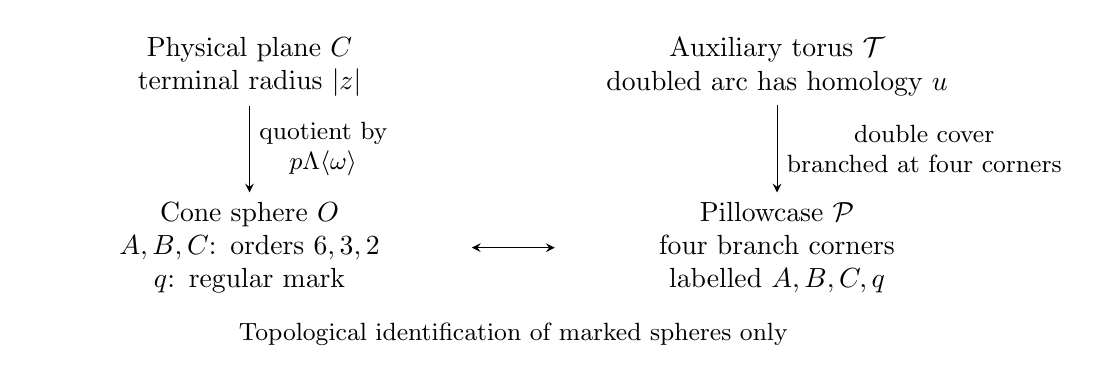
\begin{tikzpicture}[>=stealth, every node/.style={align=center}]
\node[text width=5.4cm] (physical) at (-3.35,2.3)
  {Physical plane \(\mathbb C\)\\terminal radius \(|z|\)};
\node[text width=5.4cm] (cone) at (-3.35,0)
  {Cone sphere \(O\)\\\(A,B,C\): orders \(6,3,2\)\\\(q\): regular mark};
\node[text width=5.4cm] (torus) at (3.35,2.3)
  {Auxiliary torus \(\mathcal T\)\\doubled arc has homology \(u\)};
\node[text width=5.4cm] (pillow) at (3.35,0)
  {Pillowcase \(\mathcal P\)\\four branch corners\\labelled \(A,B,C,q\)};
\draw[->] (physical) -- node[right, font=\small]
  {quotient by\\\(p\Lambda\rtimes\langle\omega\rangle\)} (cone);
\draw[->] (torus) -- node[right, font=\small]
  {double cover\\branched at four corners} (pillow);
\draw[<->] (cone.east) -- (pillow.west);
\node[font=\small] at (0,-1.1)
  {Topological identification of marked spheres only};
\end{tikzpicture}
\caption{The two covering constructions in the radius bound. The auxiliary
torus classifies the endpoint arc by a primitive vector \(u\); its physical
terminal radius is measured in the plane on the left. The identification
of the marked spheres does not identify their metrics or their covers.}
\label{fig:pv:localization-covers}
\end{figure}


Use the tetrahedral triangulation of \(O\) obtained by joining \(q\) to the
three vertices of its flag-triangle face. On \(\mathcal P\), split the two
squares by opposite diagonals, and identify corresponding triangles
affinely. Each bounded physical segment meets boundedly many period tiles
because \(p\ge1\), and boundedly many of their subdivisions. Its image in
each auxiliary triangle is a segment of bounded length. Hence the image of
\(\alpha\) has length polynomial in \(D+1\), uniformly in \(q\). This uses
bounded piece counts and triangle diameters, not a uniform derivative bound
for the affine identifications when a triangle becomes thin.

Lift \(\alpha\) in the auxiliary plane from 0 to an integer point \(u\),
whose parity is the terminal corner. The two lifts in \(\mathcal T\) form a
simple closed curve; a plane lift of this curve runs from 0 to \(2u\).
Its homology vector in the period-2 basis is thus \(u\), and
\(|u|\le (D+2)^{C_0}\) for some absolute \(C_0\). It is nonzero by parity
and primitive: a simple curve of nonzero homology on a torus is
nonseparating, and cutting along it supplies a dual curve of intersection
number one. Notice that \(u\) is not the displacement of the original
physical lift.

The straight segment from 0 to this primitive \(u\) projects to a simple
arc with the same endpoint corners. It has no internal corner, and
\((s\pm t)u\in2\mathbb Z^2\) forces \(s\pm t\in2\mathbb Z\), which rules
out any other identification of its interior points. To compare it with
\(\alpha\), take the boundary of a narrow disk neighborhood of each arc,
containing just its two endpoint marks. Each boundary lifts to a pair of
parallel torus curves of slope \(u\).

Put these two sphere boundaries in minimal transverse position relative to
the four marks. If they intersect, their number of crossings is even and at
least two. Their union has no cut vertex: after deleting any crossing, the
two remaining paths still meet at another crossing. The complementary faces
are therefore disks bounded by simple even-sided polygons, and each bigon
has distinct vertices. Euler's formula gives
\[
 \sum_{\text{faces }F}(4-\#\text{sides of }F)=8.
\]
An unmarked bigon could be removed by an isotopy. Since there are only four
marks, the formula forces exactly four bigons, each containing one mark,
and all other faces to be quadrilaterals. In the branched double cover every
marked bigon becomes a quadrilateral, while each unmarked quadrilateral
lifts to two. The resulting torus has a quadrangulation of valence four.
Gluing unit squares gives a flat torus on which the two curve families run
straight and cross perpendicularly. Its complete simply connected flat
cover develops onto the Euclidean plane; its deck maps are translations,
since they are orientation-preserving and fixed-point-free. The crossing
families consequently have different homological slopes, contradicting
their common slope \(u\).

The boundaries can thus be made disjoint. As they enclose the same pair of
marks, the annulus between them contains no mark, and they are isotopic
relative to the marks. This disk isotopy preserves terminal lift radius in
\(O\). Indeed a disk containing only an endpoint arc and the marks
\(A,q\) lifts above it to disks branched at the preimages of \(A\). In the
component about 0, the only monodromy is rotation about 0; \(q\) is regular.
All arcs in this disk from \(A\) to \(q\) therefore have equal terminal
radius. Such disk neighborhoods apply locally throughout the isotopy, and
the same observation compares the two arcs once they lie in one disk.
Thus the straight auxiliary arc has the same physical terminal radius as
\(\alpha\).

\paragraph{Reducing the shear word by cone monodromy.}
The Euclidean algorithm sends the unit horizontal vector to \(u\) by a
word in powers of the horizontal shear
\(H(x,y)=(x+y,y)\) and quarter turns, with
\(O(1+\log|u|)\) blocks. These integer linear maps act on the pillowcase.
Every shear exponent can be reduced modulo 12 without changing the terminal
physical radius of the final endpoint arc.

To see this, \(H^2\) is isotopic relative to the corners to one Dehn twist
about a curve separating them into pairs. Deform \((x,y)\mapsto(x+2y,y)\)
to \((x,y)\mapsto(x+F(y),y)\), where \(F\) is odd,
\(F(y+2)=F(y)+4\), is flat at \(2k\) near each integer row \(y=k\), and
rises by 2 between successive rows. The two twisting strips on the torus
are identified to one annulus on the pillowcase. For any curve separating
the four marks into pairs, its side containing \(q\) contains exactly one
cone mark. Its monodromy in the physical cover has order dividing 6.
Six twists consequently insert only trivial six-turn based loops at all
crossings of an endpoint arc with the twisting annulus.

When a shear block is replaced inside a word, the final arcs differ by a
conjugate of such a sixfold twist. Its supporting curve still separates the
marks into pairs, and the conjugated twist fixes each mark. This justifies
the reduction for internal blocks as well as terminal ones: the endpoint
marks remain the same at every comparison. The shortened word has length
\(O(\log(D+2))\) in a fixed finite collection of matrix maps.

\paragraph{An additive radius cost for each pure generator.}
Some matrices permute the corners, and these cannot all be lifted as maps
of the physical plane with its differently ordered cones. Separate that
permutation first. Choose fixed representatives for the matrix classes
modulo 2. If \(W=g_1\cdots g_m\) is the shortened word and \(r_i\) represents
the class of \(g_1\cdots g_i\), with \(r_0=1\), then
\[
 h_i=r_{i-1}g_i r_i^{-1},\qquad W=h_1\cdots h_m r_m.
\]
The \(h_i\) belong to a fixed finite collection of pure, corner-fixing
matrices. The representative \(r_m\) acts first on the unit arc; it has the
same corner permutation as \(W\), so the resulting arc runs from \(A\)
to \(q\). Its bounded complexity gives an initial physical radius \(O(p)\).
We do not assert a global physical-plane lift for this nonpure map.

Each pure map, transported to \(O\), does lift to a homeomorphism
\(\widetilde f\) of the physical plane fixing 0. Off the four marks, the
lifting subgroup is normally generated by the peripheral-loop powers of
orders \(6,3,2\), together with the loop about the regular mark \(q\):
upstairs these are circuits of individual punctures. A pure map preserves
these generators up to conjugacy. It therefore preserves the subgroup,
lifts off the punctures, and extends across them by the local cyclic-cover
picture.

Conjugation by \(\widetilde f\) preserves the translation subgroup of the
deck group: its nonidentity elements are exactly the infinite-order deck
transformations. Thus for a real-linear lattice automorphism \(L\),
\begin{equation}\label{eq:pv:pure-lift-equivariance}
 \widetilde f(z+\lambda)=\widetilde f(z)+L\lambda,
 \qquad \lambda\in p\Lambda.
\end{equation}
It also intertwines rotation about 0 by \(\omega\) with rotation by
\(\omega\) or \(\omega^{-1}\). Such a real-linear \(L\) is a similarity;
as it is a lattice automorphism, \(|\det L|=1\), so it is orthogonal.

The remaining bound is on one period cell, uniformly in the regular mark
\(q\). From 0 to a generic point of that cell, choose boundedly many
straight pieces in an \(O(p)\) region, avoiding lifted marks after departure.
They cross boundedly many flag triangles and their subdivisions, even when
some subtriangles are thin. After the affine identification, the path has
boundedly many bounded straight pieces in the auxiliary square model.
Applying a fixed matrix and subdividing again preserves that bound. Mapping
back, every piece lies in a physical triangle of diameter \(O(p)\), so the
path lifts to length \(O(p)\). Limits handle nongeneric points. This also
proves the bounded-complexity estimate for the initial representative arc.
It follows that \(|\widetilde f(z_0)|\le C p\) on a period cell at 0, with
one constant for the finite collection of pure generators.

Write \(z=z_0+\lambda\). Equation
\eqref{eq:pv:pure-lift-equivariance} and orthogonality now give the global
\emph{additive} bound
\[
 |\widetilde f(z)|\le |z|+C'p.
\]
Starting from the representative arc and applying the
\(O(\log(D+2))\) pure lifts, we obtain
\(D-O(1)\le Cp\log(D+2)\). Since \(p\ge1\), this proves the lemma.
\end{proof}

\subsection{Removing oversized polygons}

The geometric lemma also gives a form that will be used for polygons in a
strip. Here a pure lattice period may point in any direction; it need not
be the horizontal period of the original balanced cylinder.

\begin{corollary}\label{cor:pv:oversized-polygons}
Fix \(\delta>0\). Suppose \(\mathcal U\) is a family of planar honeycomb
polygons enclosing 0 whose interiors are disjoint from their nontrivial
translates by a common pure lattice period of length \(p\). For all
sufficiently large \(p\),
\[
 \sum_{\substack{P\in\mathcal U\\
             \max_{z\in P}|z|>p^{1+\delta}}}x_*^{|P|}=O(1).
\]
The constant is independent of the family and the period direction.
\end{corollary}

\begin{proof}
For the geometric argument, rotate coordinates to make the given period
horizontal; the six-rotation lemma is unchanged by this rotation. For the
weighted-degree argument, use an ordinary balanced cylinder in the original
lattice coordinates. Take a finite subset of oversized polygons, of mass
\(B\), and put it and all six lattice rotations into this cylinder with a
sufficiently large circumference, so that every polygon encloses one marked
face and not the other and has its original weight. This containing cylinder
need not have the given period, and its circumference may depend on the
finite subset. Lemma~\ref{lem:pv:weighted-degree} is uniform in that choice.

For two chosen polygons \(P,Q\) with area of \(P\) at least area of \(Q\),
suppose all rotations of \(Q\) are compatible with \(P\). For each rotation,
its Jordan boundary and that of \(P\) are disjoint and enclose 0, so its
closed disk lies strictly inside the disk of \(P\), by the area ordering.
The interior of \(P\) can
therefore serve as \(U\) in Lemma~\ref{lem:pv:six-rotations}, giving
\(D_Q\le Cp\log(D_Q+2)\). For fixed \(\delta>0\) and large \(p\), this
contradicts \(D_Q>p^{1+\delta}\).

The area-ordered pairs have total weight at least \(B^2/2\). Assign to each
one an incompatible rotation of \(Q\). A pair in the union with rotations
has at most six preimages, so its incompatibility numerator is at least
\(B^2/12\), while the union has mass at most \(6B\). The weighted-degree
bound gives \(B\le72r_0^{-1}\). Exhaustion by finite subsets proves the
claim.
\end{proof}

\begin{proof}[Proof of Proposition~\ref{prop:pv:planar-localization}]
On the cylinder of circumference \(p=2n\), essential polygons separating
the marked faces fall into two families, according to which cylinder end
is on the same side as each mark. Opposite families cannot coexist, and
translation by \(n\), swapping the marks, exchanges their weights. If a
finite subset of one family has mass \(B\), its union with its translated
image has mass \(2B\) and incompatibility numerator at least \(2B^2\).
Lemma~\ref{lem:pv:weighted-degree} gives \(B\le r_0^{-1}\). Thus the total
single-polygon weight of essential polygons is \(O(1)\).

Every remaining cylinder polygon is contractible. Lift its disk and
translate the enclosed marked face to 0. Its interior is disjoint from all
nonzero translates by the horizontal period \(p\). For each of the two
marked-face families, Corollary~\ref{cor:pv:oversized-polygons} shows that
the polygons whose lifted radius exceeds \(p^{1+\delta}\) have total weight
\(O(1)\).

For the upper comparison, put two independent planar disk gases of radius
\(cp\), for a fixed sufficiently small \(c>0\), around the two marked
faces. Their disks are disjoint on the cylinder, so all their polygons
qualify and
\begin{equation}\label{eq:pv:disk-cylinder-upper}
 Z(cp)^2\le F_n(2)=n^{1/6+o(1)}.
\end{equation}
For the lower comparison, remove essential and oversized polygons from a
cylinder configuration. Ignoring every avoidance restriction involving the
removed polygons bounds their possible contribution at fugacity 2 by
\[
 \prod_{P\text{ removed}}(1+2w(P))
 \le \exp\left(2\sum_{P\text{ removed}}w(P)\right)=O(1).
\]
The retained polygons lift into the two planar disk systems of radius
\(p^{1+\delta}\). Dropping restrictions between these systems yields
\begin{equation}\label{eq:pv:disk-cylinder-lower}
 F_n(2)\le C_\delta Z(p^{1+\delta})^2.
\end{equation}
The upper comparison gives exponent at most \(1/12\), and the lower one
gives exponent at least \(1/(12(1+\delta))\). Monotonicity fills the radii
between the cylinder scales. First let the radius tend to infinity for
fixed \(\delta\), then let \(\delta\downarrow0\), proving the proposition.
\end{proof}

In the strip application below, a transverse lattice period of length
comparable to the strip height makes each polygon interior period-free.
Corollary~\ref{cor:pv:oversized-polygons} therefore supplies the same
oversized-polygon removal before Proposition~\ref{prop:pv:planar-localization}
is applied to the retained disk system.
